\chapter{Preprocessing spectral data}
\label{ch:spectral_preprocessing}


\begin{wrapfigure}{o}{0.45\textwidth}
    \centering
    \vspace{-3.4cm}
    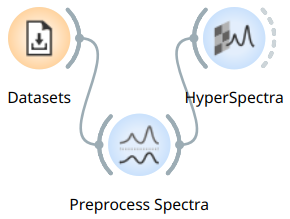
\includegraphics[width=0.45\textwidth]{workflow-preprocessing.png}
    \label{fig:spectral_preprocessing-fig1}
\end{wrapfigure}

Preprocessing spectra is a very important step of data analysis. \mutation\ has a widget, \textit{Preprocessing}, dedicated to different methods. The spectra from the ``Liver cirrhosis'' data set could use some preprocessing. There is some scattering visible and perhaps there are some artifacts due to sample thickness varying slightly.

\begin{figure}[h]
    \vspace{-0.2cm}
    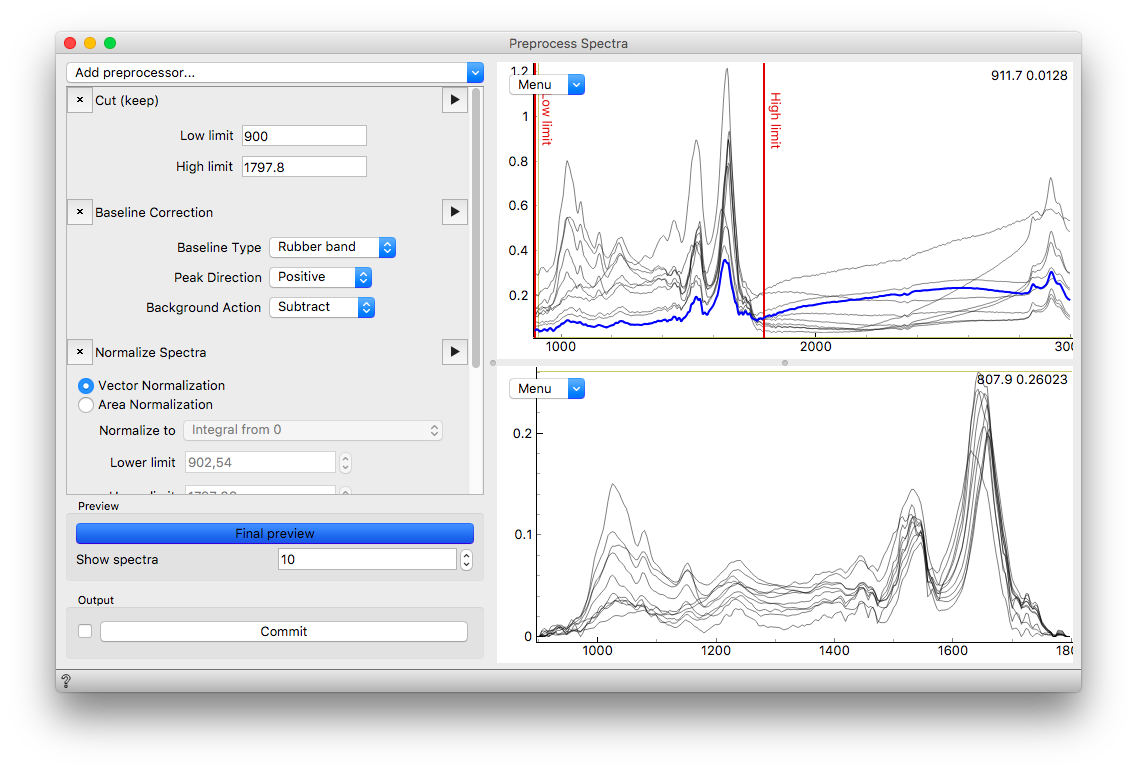
\includegraphics[scale=0.28]{spectral_preprocessing-fig2.png}
    \caption{You can add preprocessing steps from the top dropdown menu of the left panel. Then, it is possible to drag them up and down to change their order. Each preprocessor has its own parameters. In the example here we show how the Baseline correction is done: you can simply change the baseline points by dragging the red lines in the top spectrum panel. Each stage can be previewed by clicking the small triangle.}
    \label{fig:spectral_preprocessing-fig2}
\end{figure}

Let's see the result of our preprocessing in a \textit{HyperSpectra} widget.

\begin{figure}[h]
    \vspace{-0.2cm}
    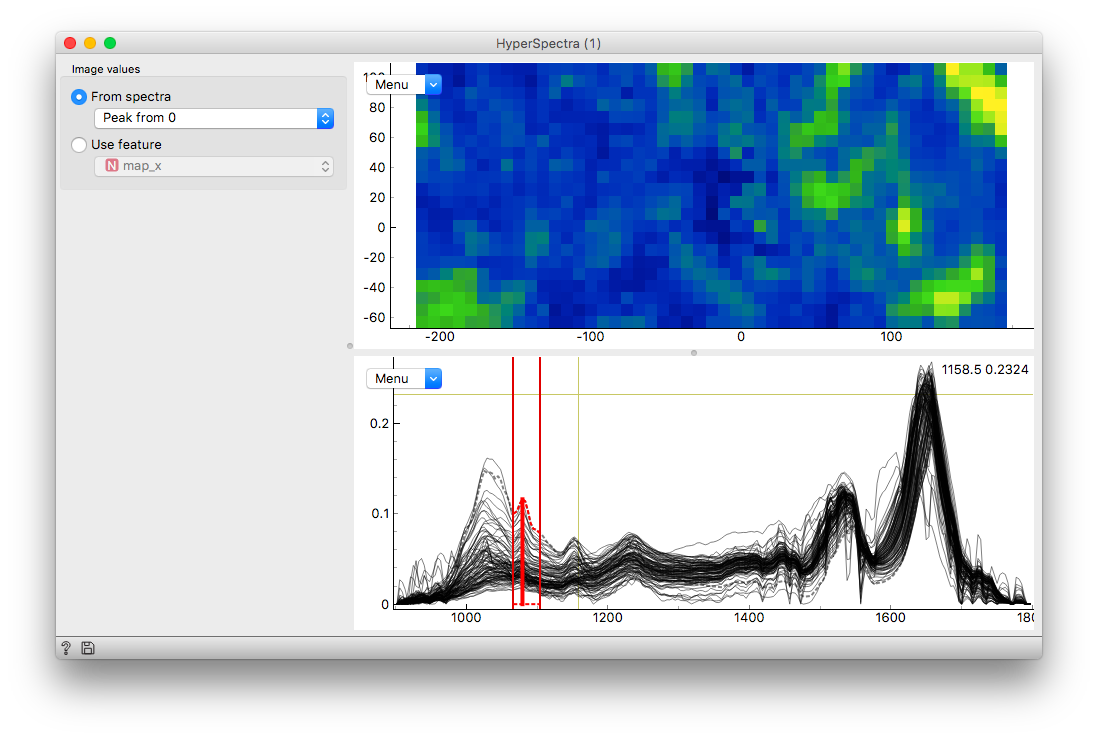
\includegraphics[scale=0.28]{spectral_preprocessing-fig3.png}
    \vspace{-1cm}
    \caption{The preprocessed data in \textit{HyperSpectra}. Did we gain anything? To investigate why the blue island disappeared, click on a pixel in it to see its spectrum.}
    \label{fig:spectral_preprocessing-fig3}
\end{figure}
